\chapter{Metodologia}

\section{Obtenção dos Dados}

Tanto para o processo de treinamento quanto para o processo de teste de uma RNA, o primeiro passo a ser dado é a obtenção das amostras experimentais para o treinamento supervisionado e teste das RNAs. Algoritmos de maquina de aprendizado supervisionados são muito mais eficazes quando treinados com conjuntos de dados muito grandes.

O primeiro passo dado nesta pesquisa foi a coleta dos dados das ondas gravitacionais. Em 1 de dezembro de 2018, o LIGO Scientific Collaboration e o Virgo Collaboration anunciaram o GWTC-1~\cite{Abbott_2019}, catálogo de ondas gravitacionais observadas pelo LIGO e Virgo durante a primeira e a segunda execução de observações, contendo os resultados completos de suas pesquisas por ondas gravitacionais, que conta com onze detecções de ondas gravitacionais provenientes dez de sistemas binários de buracos negros e um sistemas binário de estrelas de nêutrons. Como as fusões de buracos negros dominam o número de detecções de ondas gravitacionais, este trabalho focou exclusivamente neste tipo de detecção, as quais estão disponíveis no LIGO Open Science Center (LOSC)\footnote{\href{https://www.gw-openscience.org/about/}{ttps://www.gw-openscience.org/about/}}~\cite{vallisneri2015ligo}. 

Após a obtenção dos dados, foram analisados e selecionados nove das dez amostras de ondas gravitacionais de fusão de buracos negros, sendo elas: GW150914, GW151012, GW151226, GW170104, GW170608, GW170729, GW170809, GW170814, GW170823. As quais foram processadas com a ajuda da ferramenta PyCBC\footnote{\href{https://pycbc.org/}{https://pycbc.org/}}~\cite{alex_nitz_2019_2801307}, que é um pacote de software escrito em Python\footnote{\href{https://www.python.org/}{https://www.python.org/}}, usado para explorar e analisar as fontes astrofísicas de ondas gravitacionais, e capaz de detectar binários compactos coalescentes e medir seus parâmetros astrofísicos. O PyCBC contém diversos módulos para processamento de sinais e um deles é capaz de gerar formas de ondas gravitacionais. A partir desse módulo foi gerado uma forma de onda gravitacional equivalente ao formato real das ondas gravitacionais capturados pelos detectores de ondas gravitacionais (Hanford-H1 e Livingston-L1 Interferômetros) para cada uma das amostras selecionadas.

Devido aos detectores terem uma alta sensibilidade, ruídos de origens instrumentais, ambientais e provenientes de atividades humanas sempre o atingem, poluindo os sinais e dificultando as detecções. Durante todo o processo os dados oriundos do LIGO foram limpos e filtrados e também ignoradas as falhas, os blips e outras fontes de ruído de detectores transientes que dificultam a analise e processamento das ondas gravitacionais.

As formas de ondas gravitacionais são geradas como uma série temporal, usando uma das aproximações de forma de onda disponíveis pelo PyCBC. Os parâmetros principais foram as massas do sistema binário (dadas em massas solares), o tempo entre as amostras (em segundos), a frequência inicial das ondas gravitacionais (Hz) e o nome do aproximante que gostaríamos de gerar. Está disponível uma variedade de aproximações que incluem diferentes efeitos físicos. A precisão numérica depende da resolução, enquanto a precisão da extrapolação pode ser avaliada pela comparação de diferentes ordens de extrapolação. Pedidos mais altos tendem a produzir melhores resultados na fase inspiral, mas pior na fase do ringdown \cite{scharpf2017simulation}. 

Desta forma optou-se por buscar aproximadores com níveis mais elevados de precisão que tivessem o melhor resultado para ambas as parte nas simulações, devido a resultados mais atualizados e mais precisos. Para esta pesquisa foi usado o aproximante \textbf{IMRPhenomD}, pois atende altos níveis de precisão graças a uma combinação de métodos analíticos post-Newtonian (PN) e effective-one-body (EOB) para descrever a inspiração, e a calibração de modelos fenomenológicos de fusão-ringdown para simulações de relatividade numérica (NR)~\cite{khan2015frequencydomain}. Ele modela a forma de onda gravitacional nas fases de inspiração, fusão e ringdown dos buracos negros e inclui a capacidade de cada buraco negro girar na mesma direção que a órbita (rotação alinhada), atingindo bons resultados em ambas as fases de inspiral e ringdown. Além de poderem ser geradas rapidamente e para uma ampla gama de valores de parâmetros.

O PyCBC foi usado no projeto descrito nesta tese tanto para geração de banco de modelos quanto todo o processo de filtragem correspondente dos dados brutos advindos do LIGO. Usamos o PyCBC para geração simples de ondas gravitacionais no domínio da frequência com massas e tempo de amostras iguais as dos sistemas binários descritos no catalogo GWTC-1 com uma frequência inicial de 20Hz. Portanto, foram gerados nove ondas gravitacionais equivalentes as ondas gravitacionais detectadas pelo LIGO.

A escolha e adequação dos dados utilizados para treinar e testar uma RNA é de fundamental importância. É necessário que se disponha de dados em quantidade e qualidade suficientes. Caso a quantidade de dados seja pequena, a rede não conseguirá criar um modelo suficientemente representativo para se ter um desempenho satisfatório quando aplicado em situações reais após o seu desenvolvimento, o que é chamado de sobre-ajuste (overfitting) dos dados. Além disto, os dados devem englobar todos os aspectos do problema em questão, a fim de que o modelo criado seja genérico. 

Como o objetivo é treinar uma RNA que forneça um diagnóstico classificativo das ondas gravitacionais e que apresente um bom desempenho, extraímos um intervalo de 0.1 segundos de cada forma de onda com pico centralizado, deslocando a localização de pico de cada sinal aleatoriamente dentro de um intervalo de 0 a 0.05 segundos para a direita, a uma taxa de amostragem de 4096Hz. Este processo foi repetido 600 vezes para cada uma das formas de onda geradas, criando assim 5400 modelos de ondas gravitacionais, a Figura~\ref{fig:gw150914-offset} ilustra algumas das ondas geradas.

\begin{figure}[ht]
    \centerline{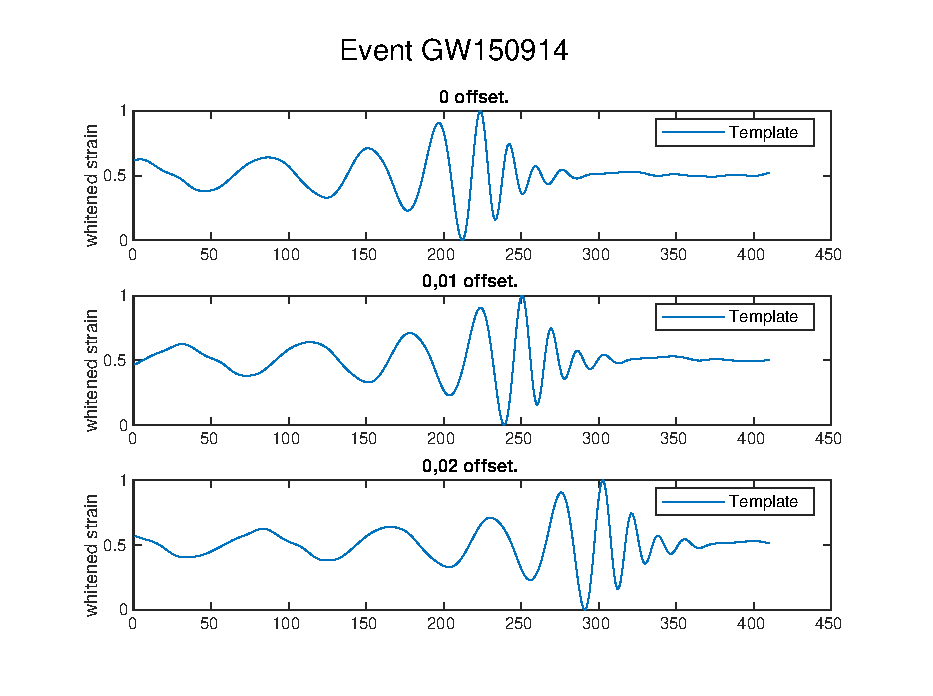
\includegraphics[width=1\textwidth]{figuras/GW150914.eps}}
    \caption{Alguns modelos de ondas gravitacionais com deslocamento}
    \label{fig:gw150914-offset}
\end{figure}

Os modelos de machine learning são construídos para minimizar erros. Desde que a probabilidade pertence a classe com maior número de observação, o algoritmo estará enviesado em classificar as novas observações. Afim de evitar o enviesamento por causa do desbalanceamento dos dados, foi criado também a mesma quantidade de amostras de ruído com espectro equivalente a densidade espectral de potência (DEP ou PSD em inglês) do ruido do LIGO~\cite{T1800044}. No final da construção dos dados, juntamos os dois bancos de dados (ruídos e modelos), totalizando o conjunto de dados de treinamento e teste com um total de 10800 amostras com duas classes: Ondas e Ruídos.

Com o objetivo de medir a performance da rede neural, é necessário avaliar a rede com um conjunto de dado que não foram previamente utilizados. Para o conjunto de dados de validação, foram necessários 2.0 segundos de observação a uma taxa amostral de 4096Hz de cada um das nove ondas gravitacionais selecionadas anteriormente, com a onda centralizada, na qual eles foram separados em várias janelas de 0.1 segundos (410 pontos) com passos de uma unidade e a mesma taxa de frequência amostral, gerando assim aproximadamente ~7780 janelas de dados. Esses dados foram gerados para os dois detectores LIGO (Hanford-H1 e Livingston-L1) separadamente, totalizando aproximadamente ~140000 dados no conjunto de validação.

Com essa imensa quantidade de dados seria difícil manter tudo sobre estruturas de arquivos simples como ".csv", pois além de consumir muito espaço físico o processo de leitura desses arquivos se tornaria demasiadamente longo. Para resolver este problema, todos os conjuntos de dados foram salvos em HDF (Hierarchical Data Format), que é uma biblioteca de software e formato de dados de alto desempenho (HDF4, HDF5) projetados para armazenar e organizar grandes quantidades de dados para facilitar a leitura dessa grande massa de dados~\cite{hdf}. Por usar árvores B para indexar os dados, o HDF funciona bem para dados de séries temporais. A maior parte dos dados entra em matrizes simples que podem ser acessadas muito mais rapidamente do que as linhas de um banco de dados SQL. 

O HDF foi desenvolvido para processamento e armazenamento de E/S rápidos de alto desempenho com um rico conjunto de recursos de desempenho integrados que permitem otimizações de tempo de acesso e espaço de armazenamento~\cite{hdf}. Esta biblioteca foi amplamente adotada em vários setores e é o padrão de fato na comunidade científica e de pesquisa, uma vez que a maioria das ferramentas que usa Machine Learning suportam esse tipo de arquivo.

Como um dos objetivos dessa pesquisa é acelerar o processo de analise das ondas gravitacionais com pouco desempenho computacionais, diversas estruturas de redes neurais do tipo MLP com diferentes parâmetros de entrada, diferentes quantidades de neurônios na camada escondida e diferentes funções de ativação foram testas visando obter a estrutura MLP a ser empregada para a detecção das ondas gravitacionais. Essa estrategia de testar varias estruturas é a prática mais recomendada e aprovada quando se deseja escolher a estrutura mais adequada~\cite{OKOH201619}.

Devido à natureza do problema, decidimos usar uma estrutura de rede neural simples para otimizar o processo de treinamento e detecção de GWs. Para implementação, execução e teste de redes neurais, o software Matlab® R2018b foi escolhido devido ao seu amplo uso pela comunidade científica.

Passamos um tempo significativo pesquisando uma ótima arquitetura de rede neural e otimizando hiperparâmetros para projetar as arquiteturas de RNA de tentativa e erro para encontrar a melhor configuração de desempenho. Para isso, muitos testes foram realizados, variando o número de neurônios na camada oculta, a taxa de aprendizado e o número de estações.

Após os testes iniciais, foi possível definir os seguintes parâmetros: uma camada oculta com 10 neurônios, 2 neurônios na camada de saída, um número máximo de 100000 iterações como critério de parada, taxa de aprendizado de 0,025, a função de transferência de todas as camadas. é linear, usamos o algoritmo Levenberg-Marquardt (trainlm) e a função de adaptação à aprendizagem (learngdm). O erro quadrático médio (MSE) foi utilizado como critério para definir o melhor resultado, pois quanto menor o MSE, melhor o resultado da rede neural. Os pesos iniciais foram gerados aleatoriamente, o que permitiu que cada rede se adaptasse a resultados diferentes dos anteriores. Além disso, restringimos as entradas a uma duração de 0,1 segundos e a uma taxa de amostragem de 4096Hz ao longo desta análise, o que é mais do que suficiente para caracterizar os eventos que estamos considerando. A Figura 1 ilustra a arquitetura da rede neural e seus parâmetros.

No processo de treinamento, o conjunto de dados de treinamento contém 10800 dados. Desses dados, 70 \% são para treinamento, 15 \% para validação e 15 \% para teste. A divisão de dados é feita aleatoriamente. O conjunto de dados para simulação contém aproximadamente ~ 70000 dados, que são usados ​​para validar a rede executando simulações com a rede treinada.

Para melhorar o processo de classificação do nosso sistema, vários RNAs foram treinados e 500 foram selecionados com o melhor desempenho e construímos uma máquina de comitê de rede neural que melhora significativamente os resultados. A máquina do comitê de rede neural desenvolvida na Figura 2 mostra um número k, em que k = 500 redes neurais treinadas individualmente de maneira independente que compartilham uma entrada comum e cuja saída individual é de alguma forma combinada. para produzir uma saída geral. As saídas dessas redes são colocadas em um módulo de combinação que executa a função de calcular a média das saídas combinadas de todas as redes neurais do comitê e apresentar o resultado semifinal do comitê de RNA.